\floatsetup[figure]{style=plain, subcapbesideposition=top}
\begin{figure}[h!]
	\centering
	\sidesubfloat[]{{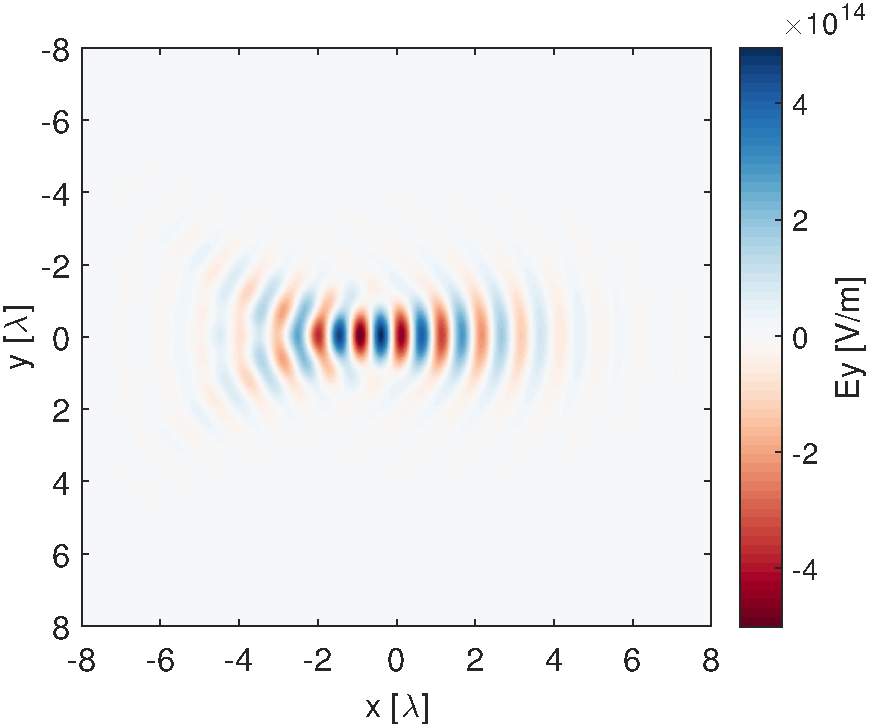
\includegraphics[width=0.44\linewidth]{./img/parax/Ey_focus.pdf}}}
	\hspace{2mm}
	\sidesubfloat[]{{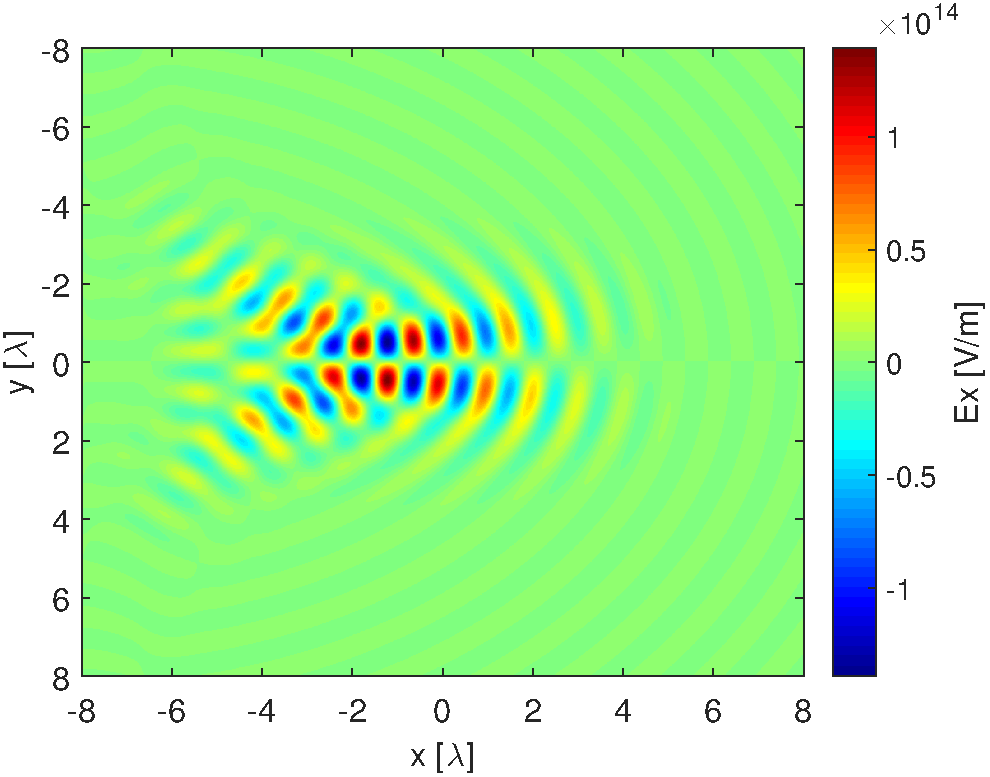
\includegraphics[width=0.44\linewidth]{./img/parax/Ex_focus.pdf}}}\\
	\sidesubfloat[]{{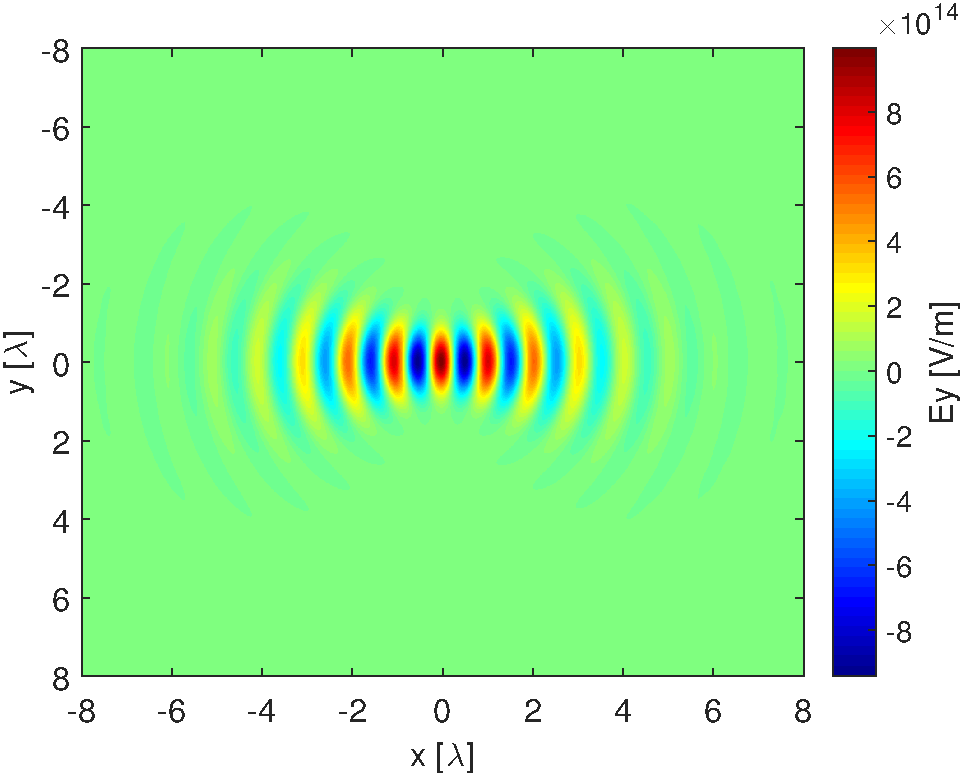
\includegraphics[width=0.44\linewidth]{./img/lbcs/Ey_focus.pdf}}}
	\hspace{2mm}
	\sidesubfloat[]{{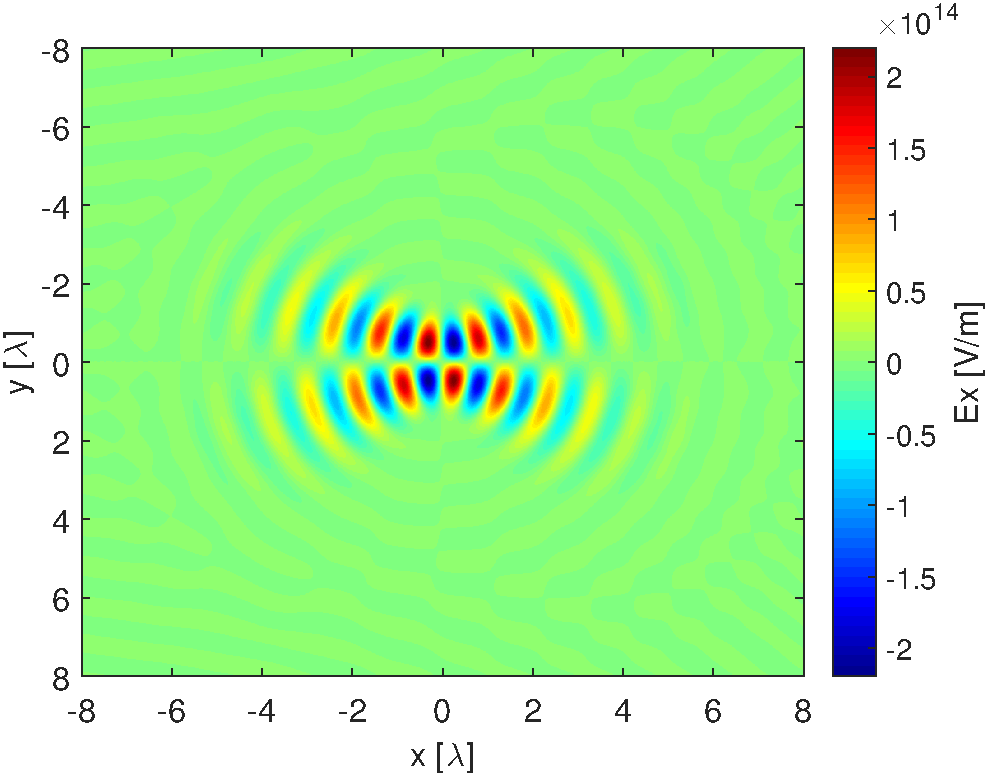
\includegraphics[width=0.44\linewidth]{./img/lbcs/Ex_focus.pdf}}}
	\caption{Transverse ($ E_{y} $) and longitudinal ($ E_{x} $) electric laser field components captured at the time step of their maximal intensity at the focal spot. The cases \textbf{(a)}, \textbf{(b)} correspond to the laser pulse initialized using the paraxial approximation, whilst \textbf{(c)}, \textbf{(d)} come from the simulation where the beam at the boundary is given by the Maxwell consistent approach. In the case of paraxial approximation, both components reveal strong distortions and asymmetry, their focal spot is located about $ \mathrm{1 \lambda} $ closer to the left boundary than specified and the corresponding amplitude is significantly lower. The laser has been attached to the left hand side boundary.}
	\label{fig:1}
\end{figure}

To evaluate the correctness of the algorithm presented in the previous section of this chapter as well as to demonstrate the drawbacks of the paraxial approximation, several test simulations in 2D geometry have been performed. In the following text, a two limit cases are presented. The first pair of simulations employs tightly focused Gaussian laser beam with the size at focus comparable with the center laser wavelength, whilst the second one shows the case of the Gaussian beam with the size at focus one order of magnitude larger than the center laser wavelength, where both approaches should return identical results. Note, that all the simulations have been computed using 2D version of PIC code EPOCH [source] instrumented with library for tight-focusing.

\floatsetup[figure]{style=plain, subcapbesideposition=top}
\begin{figure}[h!]
	\centering
	\sidesubfloat[]{{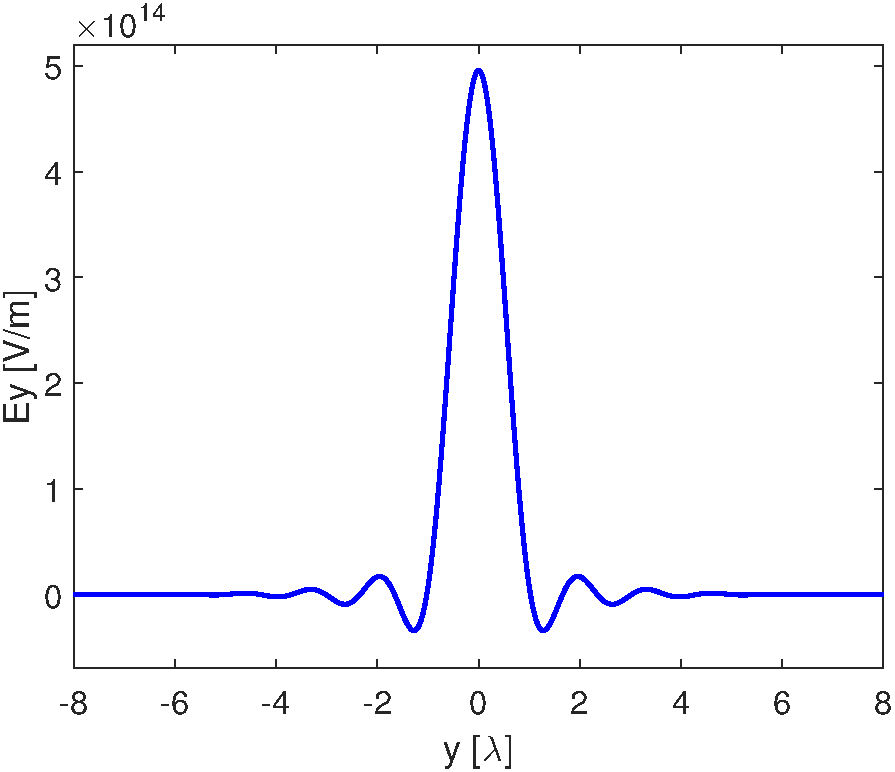
\includegraphics[width=0.4\linewidth]{./img/parax/Ey_focus_trans.pdf}}}
	\hspace{2mm}
	\sidesubfloat[]{{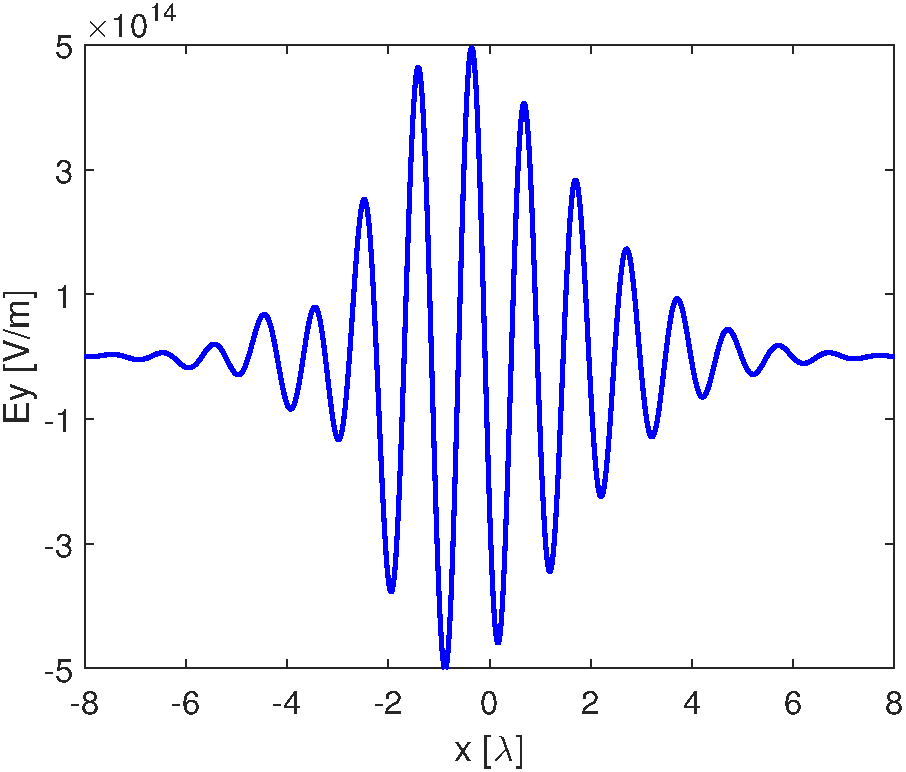
\includegraphics[width=0.4\linewidth]{./img/parax/Ey_focus_long.pdf}}}\\
	\sidesubfloat[]{{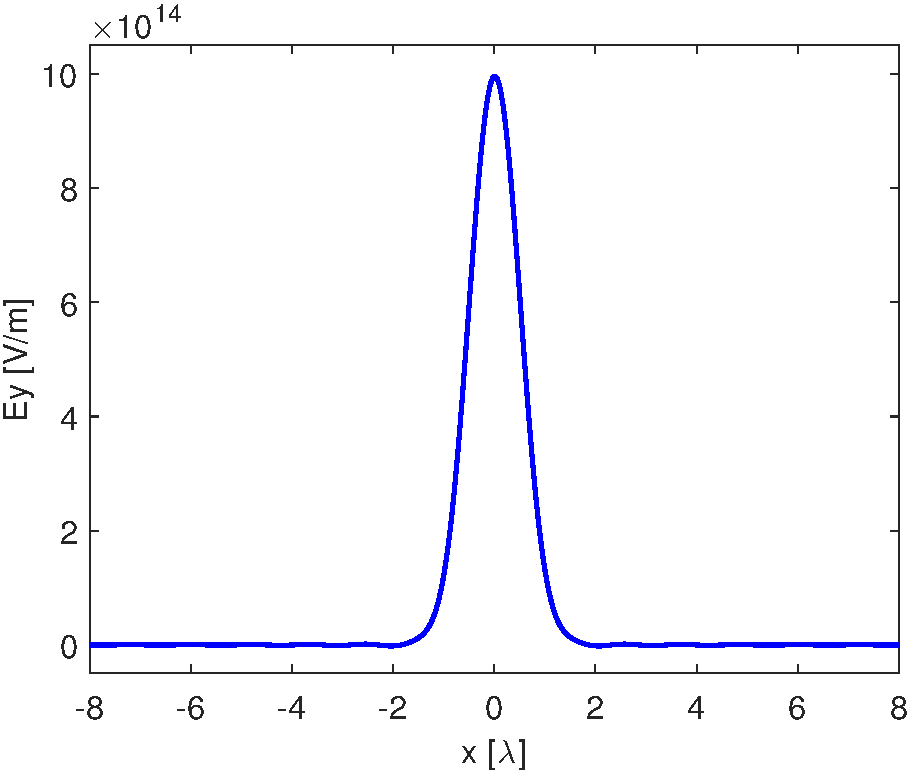
\includegraphics[width=0.4\linewidth]{./img/lbcs/Ey_focus_trans.pdf}}}
	\hspace{2mm}
	\sidesubfloat[]{{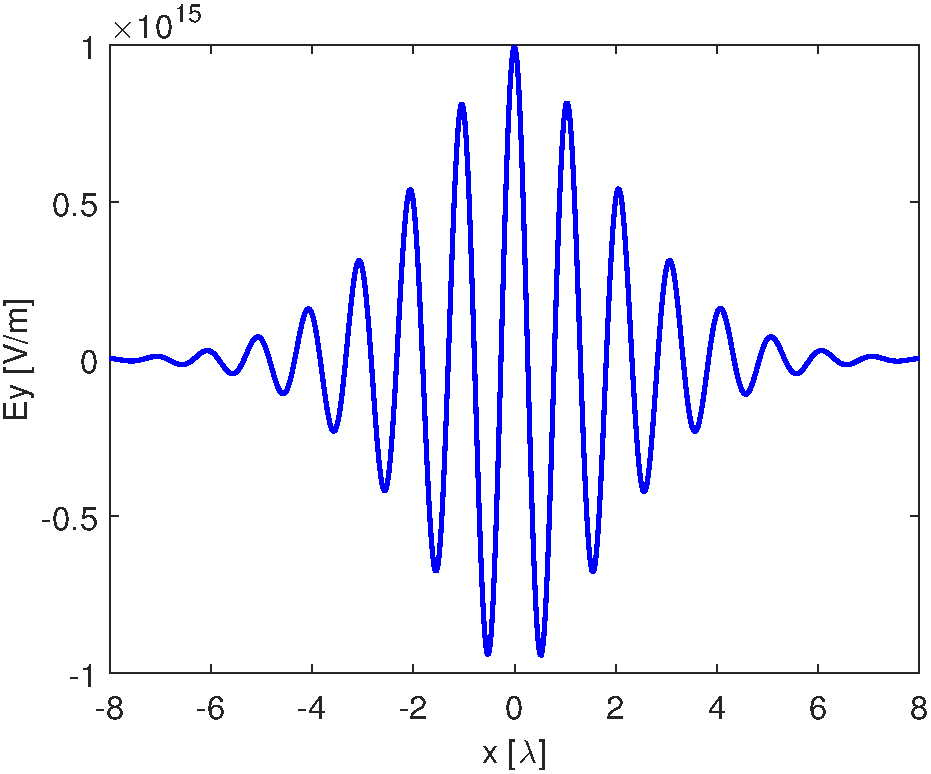
\includegraphics[width=0.4\linewidth]{./img/lbcs/Ey_focus_long.pdf}}}
	\caption{Transverse \textbf{(a)}, \textbf{(c)} and longitudinal \textbf{(b)}, \textbf{(d)} slices of the transverse electric laser field ($ E_{y} $) at the time step when it reaches maximal intensity at the focal spot. The cases \textbf{(a)}, \textbf{(b)} correspond to the laser pulse initialized using the paraxial approximation, whilst \textbf{(c)}, \textbf{(d)} come from the simulation where the beam at the boundary is given by the Maxwell consistent approach. In the case of paraxial approximation, one can clearly see strong side-wings in the spatial beam profile \textbf{(a)} as well as the asymmetry of the field in the longitudinal line-out \textbf{(b)}.}
	\label{fig:2}
\end{figure}

The simulation of a tightly focused Gaussian beam is considered first. The p-polarized laser pulse with center wavelength $ \lambda = 1 \ \mathrm{\mu m} $ propagates from left hand side boundary to the right. Its duration has been chosen to $ \tau = 20 \ \mathrm{fs} $ in FWHM and amplitude $ E_0 = 1 \cdot 10^{15} \ \mathrm{V/m} $. The beam waist $ w_0 = 0.7 \ \mathrm{\mu m} $ is shorter than the laser wavelength, which implies that non-negligible parts of $ \bar{\vec{E}}_{0, \bot}(k_x, \omega) $ are evanescent. The focus is located at a distance $ x = 8 \ \mathrm{\mu m} $ from the boundary that the laser is attached to.

The size of the simulation domain is $ 16 \lambda \times 48 \lambda $, with 100 cells per laser wavelength in both directions, thus $ \Delta x = \Delta y = \lambda/100 = 10 \ \mathrm{nm} $. The simulation time step is chosen to satisfy the CFL condition [source] $ \Delta t = 0.95 \sqrt{2} \lambda/ 100 c \approx 0.05 \ \mathrm{fs} $ and the whole simulation time is $ t = 150 \ \mathrm{fs} $. The pulse propagates in vacuum in order to get rid of all effects that could be potentially caused by plasma. All the simulation parameters can be found in the attached input files in the appendix A.

\floatsetup[figure]{style=plain, subcapbesideposition=top}
\begin{figure}[h!]
	\centering
	\sidesubfloat[]{{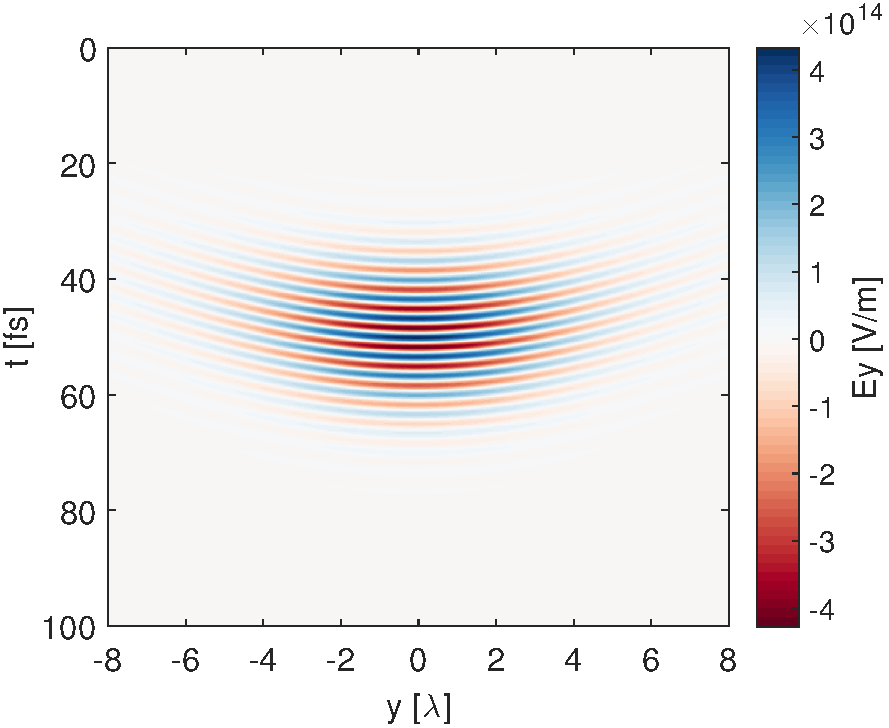
\includegraphics[width=0.44\linewidth]{./img/lbcs/Ey_boundary_time.pdf}}}
	\hspace{2mm}
	\sidesubfloat[]{{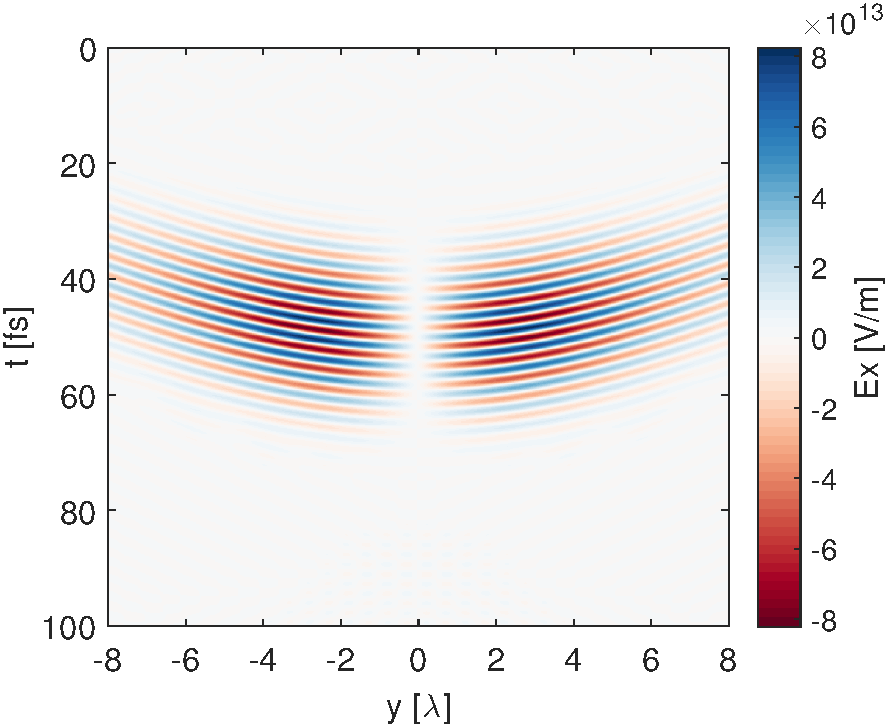
\includegraphics[width=0.44\linewidth]{./img/lbcs/Ex_boundary_time.pdf}}}
	\caption{The time evolution of transverse ($ E_{y} $) \textbf{(a)} and longitudinal ($ E_{x} $) \textbf{(b)} electric laser field components at the boundary that the laser is attached to. Both components has been calculated according to the Maxwell consistent approach.}
	\label{fig:3}
\end{figure}

\begin{figure}[h!]
	\centering
	\sidesubfloat[]{{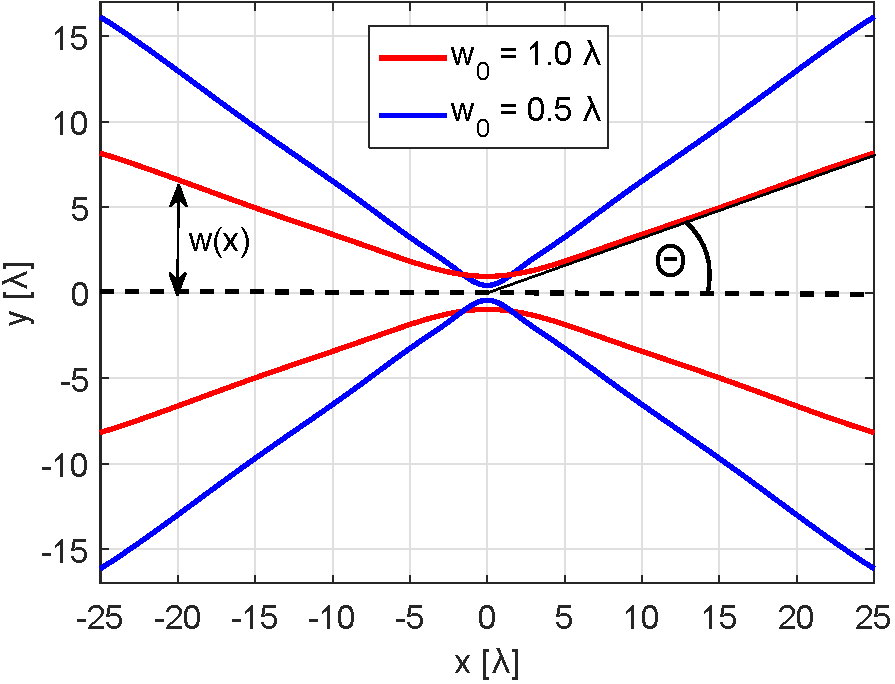
\includegraphics[width=0.45\linewidth]{./img/lbcs/divergence.pdf}}}
	\hspace{2mm}
	\sidesubfloat[]{{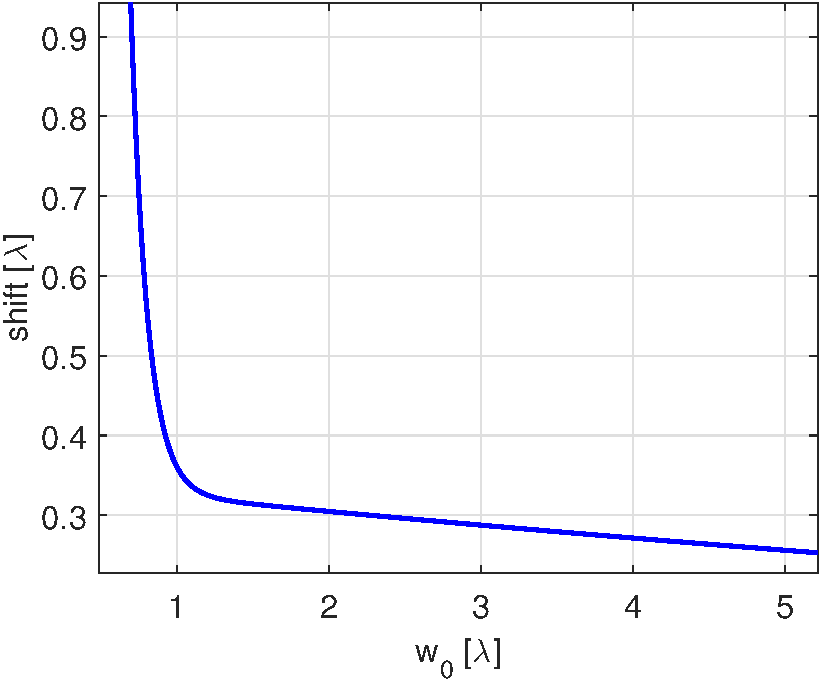
\includegraphics[width=0.43\linewidth]{./img/parax/focus_shift.pdf}}}
	\caption{\textbf{(a)} Graph of the spot size parameter $ w(x) $ of the beams with $ w_0 = 1 \: \lambda $ and $ 0.5 \: \lambda $ calculated using Maxwell consistent approach. From the plotted lines, one can roughly estimate the beam divergence angle $ \Theta $. The divergence angles for both beams are surprisingly in a good accordance with the formula for divergence angles of corresponding Gaussian beams. \textbf{(b)} Dependency of the absolute focal point shift on the beam waist $ w_0 $ for the laser beam initialized using the paraxial approximation. One can see sharp increase of the error for $ w_0 < \lambda $. In both cases, values have been dumped at discrete time intervals and interpolated.}
	\label{fig:7}
\end{figure}

\floatsetup[figure]{style=plain, subcapbesideposition=top}
\begin{figure}[h!]
	\centering
	\sidesubfloat[]{{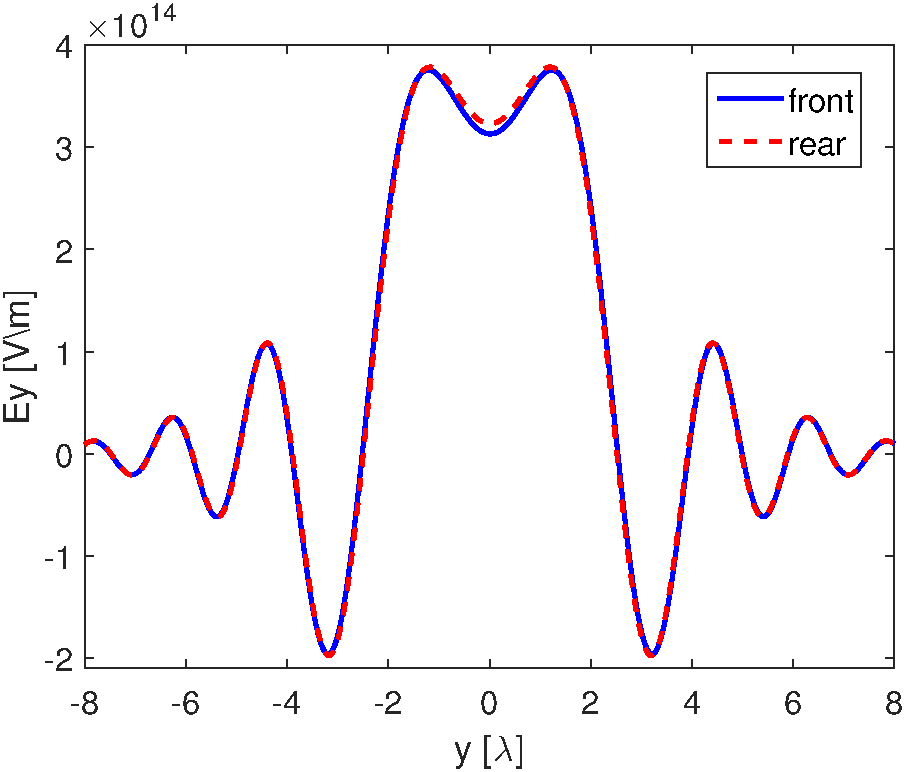
\includegraphics[width=0.44\linewidth]{./img/lbcs/Ey_boundary_trans.pdf}}}
	\hspace{1mm}
	\sidesubfloat[]{{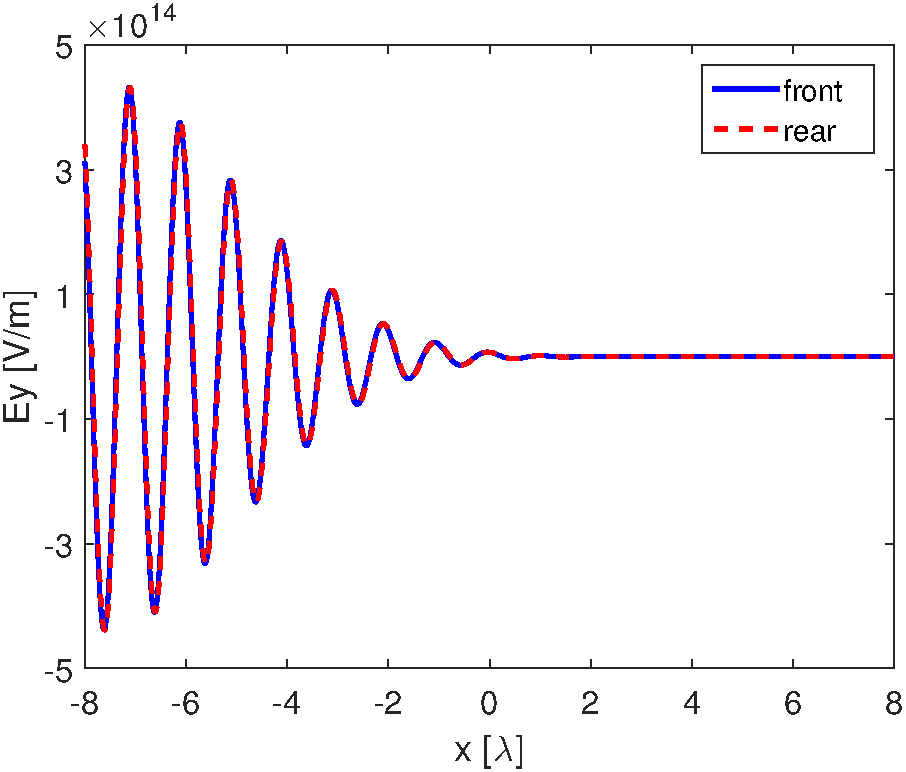
\includegraphics[width=0.44\linewidth]{./img/lbcs/Ey_boundary_long.pdf}}}
	\caption{Transverse \textbf{(a)} and longitudinal \textbf{(b)} slice of the transverse electric laser field ($ E_{y} $) when it reaches its maximal intensity at the front (blue) and rear (red) boundary. The results come from the simulation where the laser beam at the boundary has been calculated using the Maxwell consistent approach. For better comparison, the field at the rear boundary in \textbf{(b)} has been horizontally flipped. The exact match between the field shapes at a different time steps of simulation proves the correctness of the laser beam propagation.}
	\label{fig:4}
\end{figure}

In the following paragraph, the results of the first simulation are discussed in more details. Fig. \ref{fig:1} shows the transverse and longitudinal electric field components at their maximal intensity at focus for two cases. First, for the laser beam which has been initialized using the paraxial approximation (fig. \ref{fig:1}-a, \ref{fig:1}-b), i.e. the electric field at the boundary is given by the equation \ref{1.50}, and second, according to the approach consistent with the Maxwell's equations (fig. \ref{fig:1}-c, \ref{fig:1}-d). In the case of paraxial approximation, one can clearly see strong distortions and asymmetry in the shape of both electric field components. In addition, the focus location is shifted about $ 1 \ \mathrm{\mu m} $ closer to the left boundary and the corresponding amplitude at focus is less than half the required value. In contrast, the fields produced by the simulation using Maxwell consistent calculation of laser fields at boundary are symmetric with respect to the focal spot and without any distortions. Furthermore, the focus location as well as the amplitude fulfills the initial requirements precisely.

Fig. \ref{fig:2} shows transverse and longitudinal slices of transverse electric field component at focus for the case of the laser beam initialized using the paraxial approximation (fig. \ref{fig:2}-a, \ref{fig:2}-b) as well as for the case where the beam at the boundary is given by the Maxwell consistent approach (fig. \ref{fig:2}-c, \ref{fig:2}-d). For the case of paraxial approximation, one can clearly see the asymmetry of the field shape in the longitudinal slice (fig. \ref{fig:2}-b), which consequently leads to a decrease of the amplitude at focus and to the strong side-wings in the spatial beam profile, as might be better seen from the transverse slice (fig. \ref{fig:2}-a). On the other hand, Maxwell consistent approach calculates fields of perfect symmetry with respect to the focal spot (fig. \ref{fig:2}-c) and no side-wings or distortions are present (fig. \ref{fig:2}-d).

\begin{figure}[h!]
	\centering
	\sidesubfloat[]{{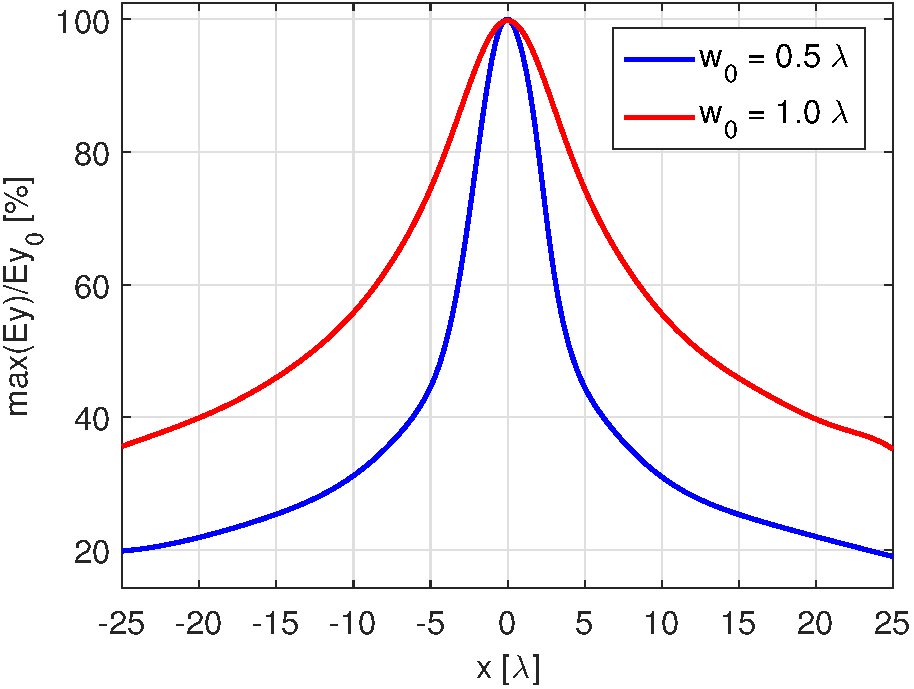
\includegraphics[width=0.445\linewidth]{./img/lbcs/amplitude.pdf}}}
	\hspace{2mm}
	\sidesubfloat[]{{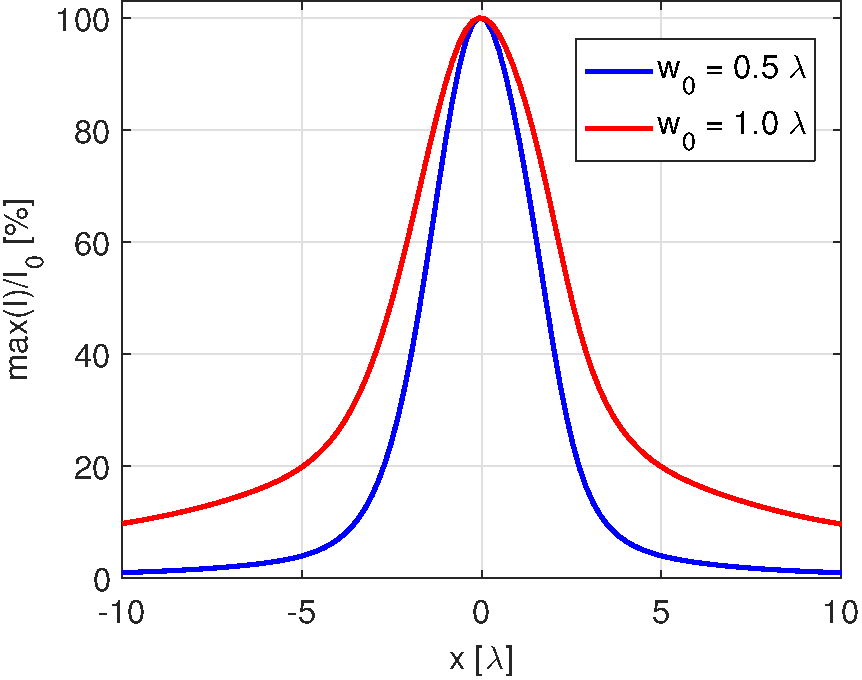
\includegraphics[width=0.435\linewidth]{./img/lbcs/intensity.pdf}}}
	\caption{\textbf{(a)} Graph of the transverse ($ E_{y} $) electric laser field amplitude with respect to the distance from the focal spot. The values on vertical axis are given in a percentage of the amplitude at focus $ E_{y, 0} $. \textbf{(b)} Graph of the maximal instantaneous laser intensity with respect to the distance from focal spot. The values on vertical axis are given in a percentage of the laser intensity at focus $ I_{0} $. In both cases, values have been computed using the Maxwell consistent approach, dumped at discrete time intervals and interpolated.}
	\label{fig:8}
\end{figure}

\floatsetup[figure]{style=plain, subcapbesideposition=top}
\begin{figure}[h!]
	\centering
	\sidesubfloat[]{{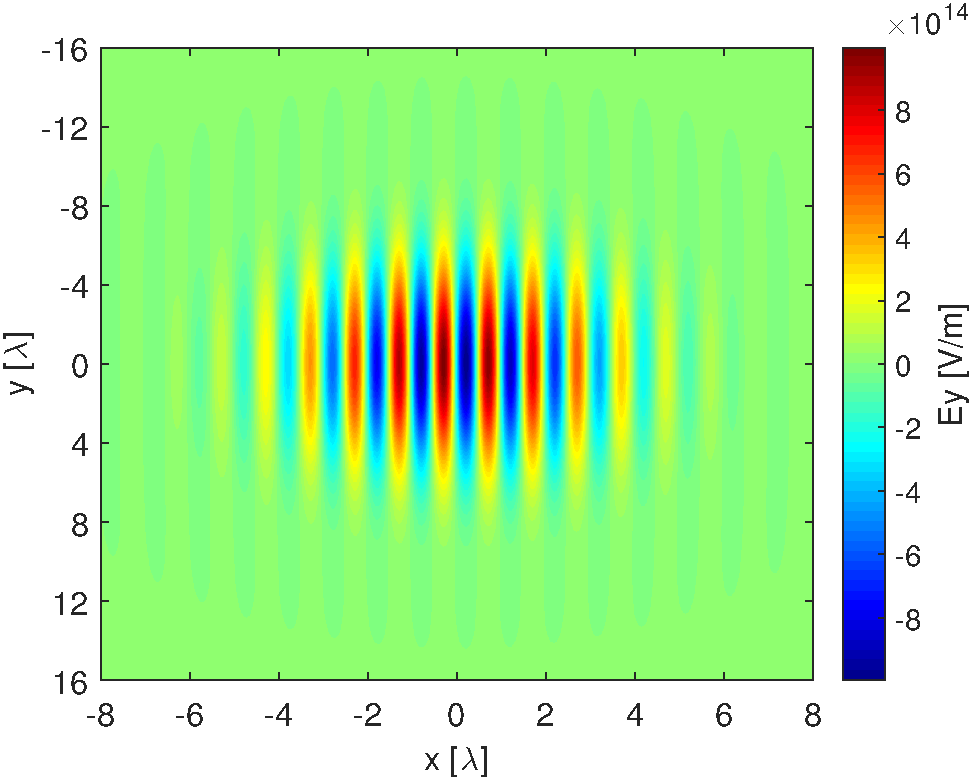
\includegraphics[width=0.45\linewidth]{./img/parax/Ey_focus_5mic.pdf}}}
	\hspace{2mm}
	\sidesubfloat[]{{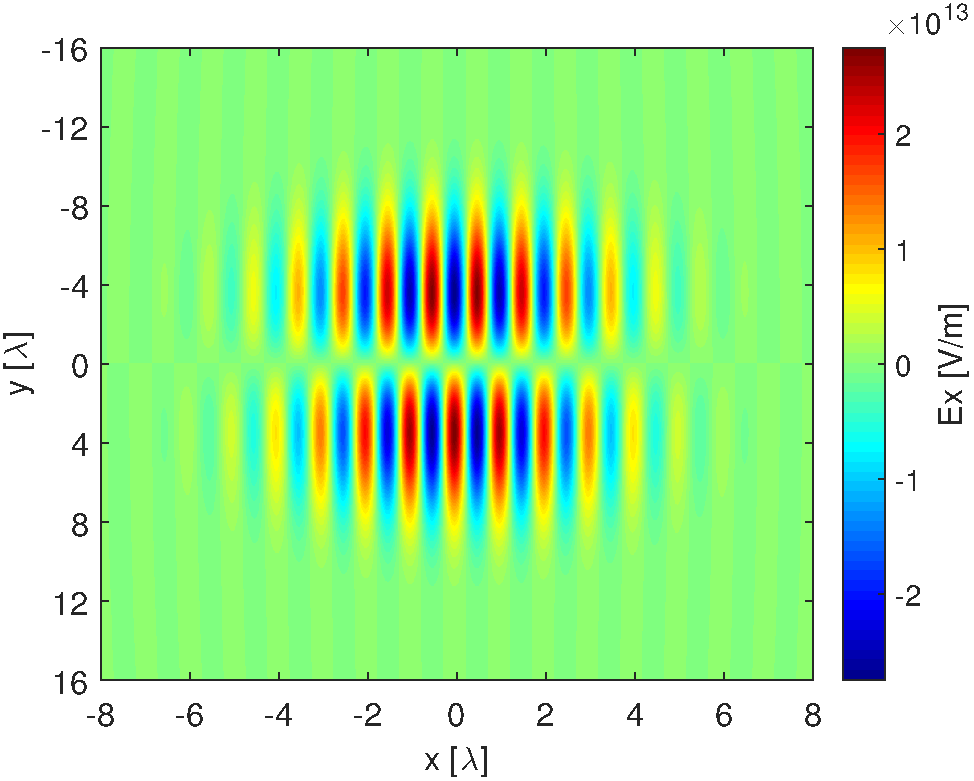
\includegraphics[width=0.44\linewidth]{./img/parax/Ex_focus_5mic.pdf}}}\\
	\sidesubfloat[]{{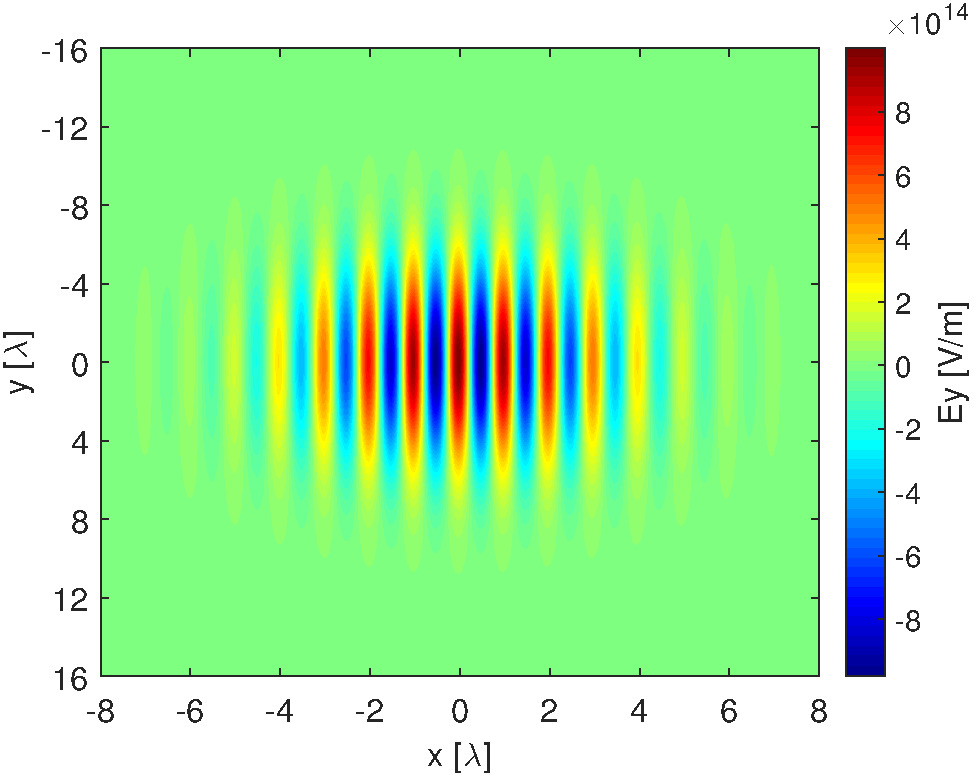
\includegraphics[width=0.44\linewidth]{./img/lbcs/Ey_focus_5mic.pdf}}}
	\hspace{2mm}
	\sidesubfloat[]{{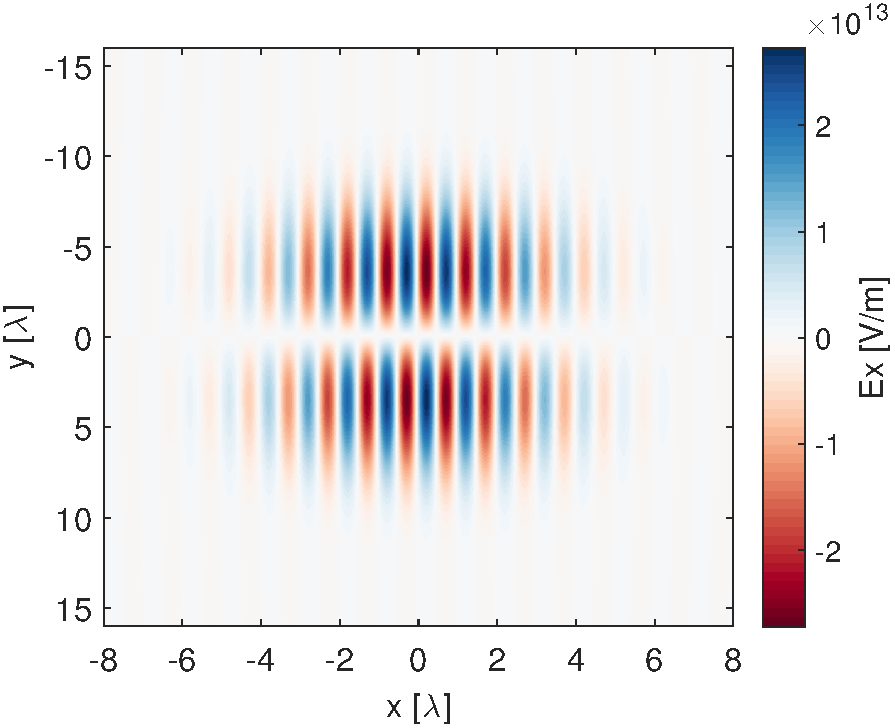
\includegraphics[width=0.43\linewidth]{./img/lbcs/Ex_focus_5mic.pdf}}}
	\caption{Transverse ($ E_{y} $) and longitudinal ($ E_{x} $) electric laser field components captured at the time step of their maximal intensity at the focal spot. The cases \textbf{(a)}, \textbf{(b)} correspond to the laser pulse initialized using the paraxial approximation, whilst \textbf{(c)}, \textbf{(d)} come from the simulation where the beam at the boundary is given by the Maxwell consistent approach. The size of the focus has been chosen to be one order of the magnitude larger than the center laser wavelength. One can clearly see, that there is no significant difference between the shapes of the electric field components.}
	\label{fig:5}
\end{figure}

\floatsetup[figure]{style=plain, subcapbesideposition=top}
\begin{figure}[h!]
	\centering
	\sidesubfloat[]{{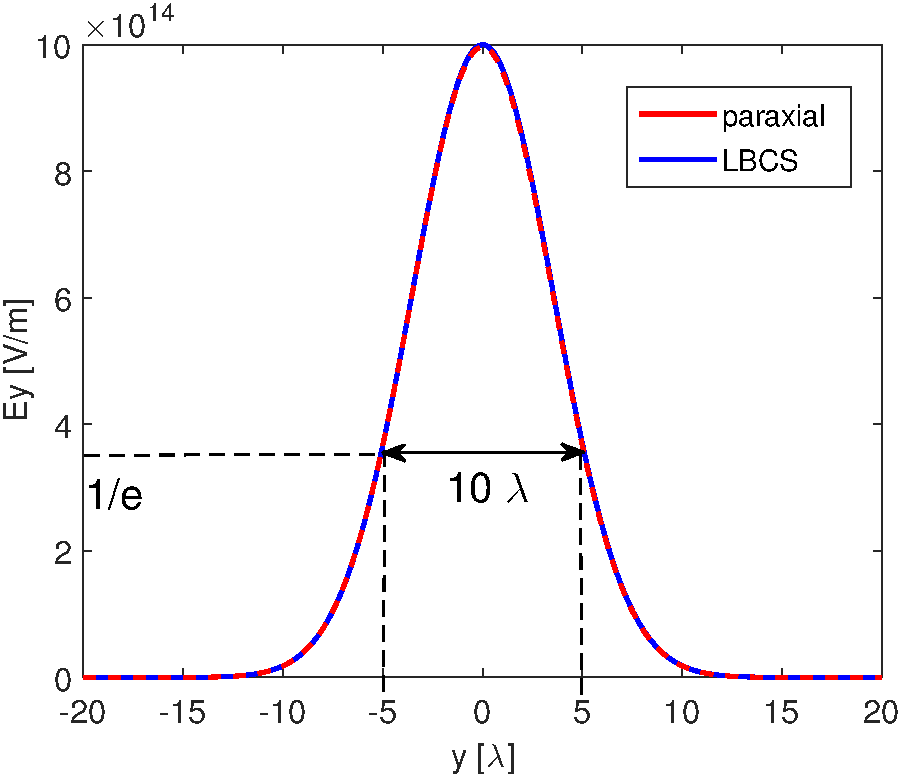
\includegraphics[width=0.44\linewidth]{./img/parax/Ey_focus_trans_comparison.pdf}}}
	\hspace{2mm}
	\sidesubfloat[]{{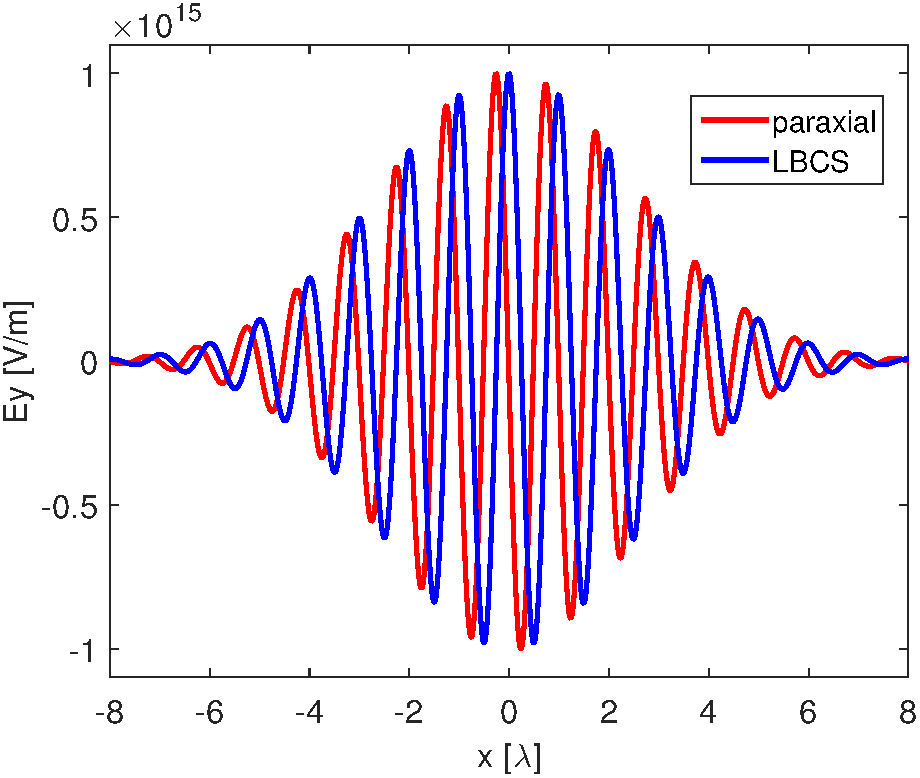
\includegraphics[width=0.44\linewidth]{./img/parax/Ey_focus_long_comparison.pdf}}}
	\caption{Transverse \textbf{(a)} and longitudinal \textbf{(b)} slices of the transverse electric laser field ($ E_{y} $) at the time step when it reaches maximal intensity at focus. Red lines correspond to the laser pulse initialized using the paraxial approximation, whilst blue lines come from the simulation where the beam at the boundary is calculated by the Maxwell consistent approach (LBCS). The size of the focus has been chosen to be one order of magnitude larger than the center laser wavelength. In the case of paraxial approximation, the focus is slightly shifted closer to the left boundary \textbf{(b)}, otherwise the size of the focus as well as the amplitude is correct for both cases \textbf{(a)}.}
	\label{fig:6}
\end{figure}

In fig. \ref{fig:3} one can look through the time evolution of transverse (fig. \ref{fig:3}-a) and longitudinal (fig. \ref{fig:3}-b) electric field components at the boundary as computed using the Maxwell consistent approach. Note that one must chose carefully the transverse size of the domain, since the beam width at boundary may be much larger than at focus because of a diffraction. To estimate the beam width at the boundary, one has to know the beam divergence angle $ \Theta $. In fig. \ref{fig:7}-a, one can find a graph of the spot size parameter $ w $ as calculated using the Maxwell consistent approach for the beams focused to $ w_0 = 1 \ \lambda $ and $ 0.5 \ \lambda $. From the plotted lines, one can roughly estimate the beam divergence angle $ \Theta $. For the beam focused to $ w_0 = 1 \ \lambda $, the beam divergence angle has been around $ \Theta = 18.2^{\circ} $ which is almost identical value as for the Gaussian beam of the same parameters. For the beam with $ w_0 = 0.5 \ \lambda $ the divergence has been estimated to $ \Theta = 32.9^{\circ} $, while the Gaussian beam with the same size at focus has divergence $ \Theta = 36.5^{\circ} $. Consequently, in spite of the fact that the divergence of the tightly focused beams calculated using the Maxwell consistent approach is a little bit lower, both approaches are in quite a good accordance regarding this parameter and one can use the angle $ \Theta $ given by the equation \ref{1.38} as a rough estimate even for tight-focusing.

To evaluate a correctness of the propagation of the beam prescribed using the Maxwell consistent approach, several criteria has been defined. The correctness of the amplitude and beam waist as well as the right focus location has already been verified. Additional criteria has been set on a beam symmetry. In fig. \ref{fig:4}, one can find a comparison of the transverse electric laser field component when it achieves its maximal intensity at front and rear boundary. One can clearly see the exact match between the field shapes at different time steps of the simulation in transverse (fig. \ref{fig:4}-a) and longitudinal (fig. \ref{fig:4}-b) slices. Moreover, all the aforementioned criteria has been fulfilled also in other simulations with different input parameters that are not presented here. Consequently, these observations prove the correctness of the simulation at least for the tightly focused Gaussian laser beams.

In fig. \ref{fig:7}-b, one may find the estimate of the absolute focal point shift with respect to the prescribed position of the beam waist. The interpolated values come from the simulations where the laser beam has been initialized using paraxial approximation. One can clearly see the sharp increase of the error for $ w_0 < \lambda $. On the other hand, for $ w_0 = 5 \ \lambda $ the shift is around $ 0.2 \ \lambda $ which is negligible in comparison with the Rayleigh range.

In fig. \ref{fig:8}-a, one can see the amplitude of the transverse electric laser field with respect to the distance from the focal spot calculated using Maxwell consistent approach. This could be particularly useful for experiments since it is not always easy to focus the beam onto the target surface perfectly. Sometimes, one might be more interested in the laser intensity rather than the amplitude of the electric field. For this reason, fig. \ref{fig:8}-b shows the instantaneous maximal laser intensity in the narrower spatial interval calculated from the values of the electric field amplitude.

Up to now, we have demonstrated the results of simulations with tight-focusing. In the following, comparison of the two numerical methods for the beam focused to a larger spot size characterized by $ w_0 = 5 \ \lambda $ is presented. Except for the beam waist, all the input parameters remained the same. The parameter $ w_0 = 5 \ \lambda $ is about the limit case for the beam initialized using the paraxial approximation. Thus, one expects that the simulation results of both methods should be almost identical.

Similarly as in fig. \ref{fig:1}, fig. \ref{fig:5} shows again transverse and longitudinal electric field components at their maximal intensity at focus for both cases, laser beam initialized using the paraxial approximation (fig. \ref{fig:5}-a, \ref{fig:5}-b) and according to the approach consistent with the Maxwell's equations (fig. \ref{fig:5}-c, \ref{fig:5}-d). Here, one cannot register any difference between the results corresponding to both approaches. Also, the transverse slice of the transverse electric laser field component at focus (fig. \ref{fig:6}-a) shows the correct shape and amplitude for both cases. The longitudinal slice (fig. \ref{fig:6}-b), however, points out the fact that the location of the focal spot is still a little bit shifted closer to the left hand side boundary. Nevertheless, this difference could be neglected in practice. At the end of the day, the beam diameter at focus should be at least one order of magnitude larger than the center laser wavelength for the Gaussian beams propagating in the paraxial approximation.

In conclusion, one should be aware that the propagation of tightly focused laser pulses cannot be described by paraxial approximation. It has been shown above that for the beams focused to a spot with the size comparable to a center laser wavelength, paraxial approximation leads to a shifted location of the focus, asymmetric laser field profiles with distortions and lower amplitude. These deviations are far from negligible and have without doubt a strong impact on the laser-matter or laser-plasma interaction results. On the other hand, the propagation of tightly focused Gaussian laser beams prescribed at boundaries according to the Maxwell consistent approach has been proven to be correct.

It has been also verified that the paraxial approximation can be safely used when the beam size at focus is about one order of magnitude larger than the center laser wavelength, such that $ w_0 \geq 5 \ \lambda $. In this case, the laser fields are symmetric with respect to the focal point, the laser intensity fulfills specified requirements precisely, only the location of the focus is shifted about $ 0.2 \ \lambda $ closer to the boundary at which the laser is attached to. However, in this case, the simulations generally produce physically relevant results, therefore the effect of the focal point shift can be neglected in practice.

Regarding the validity and trustworthiness of simulation results, no exact threshold for the size of the focal spot for laser beams initialized using the paraxial approximation has been determined. The rate of unphysical effects also depends on investigated phenomena and other laser pulse properties, such as intensity or duration. Thus the frequently used simulation set-up for beams with the waist $ w_0 = 3 \ \lambda $ can be in many situations justified.